\documentclass[12pt]{scrreprt}
\newcommand{\tab}{\hspace*{2em}}
\usepackage[english]{babel}
\usepackage[utf8]{inputenc}
\usepackage{graphicx}
\usepackage{mathtools}
\usepackage{pdfpages}
\graphicspath{ {images/} }


\title{Pascal Compiler}

\author{Ken Johnson}
\date{December 18, 2014}

\begin{document}
\maketitle

\tableofcontents

\chapter{Introduction}
This document is an overview of the design process and implementation of a Pascal 
 Compiler written in Java. The compiler takes an input Pascal file, and compiles to MIPS
 assembly language. The following sections contain a brief ovew of the entire
 process of the compilation, followed by an in depth explanation of each component is
 given in the chapters following the overview. The explanations of design decisions
 are somewhat minimal, as the majority of the decisions for the first two
 components of the compiler were primarily a direct result of instruction, and 
 the specifications given. As a note, there are a few things in the grammar that 
are not fully implemented in the compiler: the or and and operations are not functional
as well and scientific notation. Functions, procedures, and arrays were all also left
out of the functionality of the compiler.
\chapter{Overview}
To compile the Pascal code there are a variety of components the compiler must consist
 of; these will be discussed in short here.
\section{Scanner}
The scanner is the first phase of the compilation process. The scanner's purpose is to scan
through the input file, and analyze its contents character by character to build up tokens.
 The tokens are the accepted keywords of the language, IDs, numbers, etc. A full list of 
 these tokens can be found in the Scanner chapter, and in Appendix A in the full grammar 
 specification of the language.

\section{Recognizer}
The next phase of the compiler is the recognizer. In a the final product this will be a 
full parser instead of just a recognizer. The recognizer uses the grammar found in Appendix 
A to analyze the tokens found using the scanner. This analysis determines whether the 
Pascal code will compile or not according to the grammar. If the code is correct and 
will compile, the compiler will print out a success message and exit with code 0. If there 
is an error it will state the line on which the error occurred and exit with a code 
corresponding to the error. These codes can be found in Appendix B.
\section{Parser}
The Recognizer has been exteded to a full parser. The purpose of the parser to perform
all the same functions as the recognizer, but it now also creates a symbol table and
a syntax tree. The implementation of this is a recursive descent parser.
\subsection{Symbol Table}
The symbol table hold all declared variables, functions, and procedures, as well as 
their types.

\subsection{Syntax Tree}
The syntax tree is simply an internal representation of the pascal code. It consists of
nodes, starting from the root Program node.

\section{Code Generator}
The Code Generator is the piece of the compiler that will translate the internal representation
of the code to assembly. It is given a Syntax Tree, and it generates non-optimized MIPS
Assembly code.

\chapter{Scanner}
The scanner will be discussed in more depth here. The input is handled by a PushbackReader 
in order to push unwanted characters back in to the input stream. The scanner consists of 
this PushbackReader, a TransitionTable, an enum of tokens, and a SymbolTable. This 
TransitionTable is the corresponding table for the DFA found in Appendix C. Character by 
character the table appends to a working string (built with a StringBuilder), according to 
the current state and the next state. For example:
Given the line\\* 
\begin{center}
\textit{var x :=}\\*
\end{center}
the scanner would step through starting with \textit{v}, seeing that it is a letter, it 
moves into the ID state. The scanner then appends the \textit{v} to working string which 
was previously $\lambda$. It will then repeat the same process with \textit{a} and 
\textit{r}. Once the reader reaches the space it will push this back, and accept the token.
 Next it checks to see if \textit{var} is in the SymbolTable. The SymbolTable has a value 
for \textit{var} that is equal to Token.VAR. Since the symbol was recognized, the token 
value is now Token.VAR. The space is then passed over, moving to the \textit{x}. The 
\textit{x} is appended to the $\lambda$ string and the space is pushed back. The string is 
checked against the SymbolTable, and nothing is found so the token returned it Token.ID. 
Next the \textit{:} is brought in by the parser. This has its own state as \textit{:} is a 
valid symbol, as is \textit{:=}. The scanner now appends the \textit{:} to the $\lambda$ 
string and moves to the next state. Since the next character is \textit{=} is appends this 
and moves to the symbol acceptance state. There is no need to push anything back here, as 
nothing else appended to this is a valid token, and the check for the validity of the token
 ordering is done later in the parser/recognizer. This is also queried against the 
 SymbolTable and is assigned the value Token.ASSIGNOP. Granted this is not a valid line of 
 Pascal code, but according to the scanner, it works.
\chapter{Recognizer}
The recognizer, which will later be a full-fledged parser, is the second layer of the 
compiler. It uses the tokens from the scanner to parse the syntax of the Pascal file. This 
is done by almost directly implementing the grammar specified in Appendix A. Each of the
non terminals in the grammar corresponds to the same method in the recognizer. For example 
take the first rule in the grammar: \\*
\textit{program} $\rightarrow$ \tab\hspace{4mm}\textit{\textbf{program id ;}}\\*
\tab\tab\tab\tab\textit{declarations}\\*
\tab\tab\tab\tab\textit{subprogram\_declarations}\\*
\tab\tab\tab\tab\textit{compound\_statement}\\*
\tab\tab\tab\tab\textit{\textbf{.}}\\*
This is of course the first thing that must be in a Pascal file. The first token must be 
program, followed by an id and a semicolon. This is checked in the \textit{program} method 
in the recognizer. As these are bold in the grammar, they represent tokens. The following 
non-bold rules are other non-terminals. Because of this the \textit{program} method calls 
the \textit{declarations} method, which will in turn match tokens \textit{var} and then 
call \textit{identifier\_list}, which in turn calls other methods. After moving back up the
stack of calls from \textit{declarations} program calls \textit{subprogram\_declarations} 
and repeats the process before moving on to \textit{compound\_statement}. The program then 
matches the . or the PERIOD token. This is the parsing of the entire file, 
as everything is contained between the \textit{program} and the PERIOD and parsed 
further down the call stack. The recognizer checks to make sure that there are no issues in
 parsing and then prints a success message. It does not yet assign any meaning to the 
syntax, this will be handled by the actual parser. If there is an error found while parsing
the file, it shows the line it encountered the error, and what type of error occurred. A 
full list of these errors and error codes can be found in Appendix B. 

\chapter{Parser}
The extension of the recognizer discussed in the previous section, works as a recursive
descent parser. As the lexical tokens were previously recognized, they are now parsed and
assigned meaning. This means that the parser starts at Program, then recursively goes
over the remainig parts of the program. During the declarations part of the parsing, symbols
are added to the Symbol Table. The information added here is what kind of declaration it is,
var, array, procedure, or function, the type of value or return value, and its lexical
token. It also handles the various scopes used by different methods. This is used to ensure
variables have been declared. No instantiation is required to use a variable, but values
default to zero. As of this moment, functions, procedures and arrays are recognized, and to
some extent put into the Symbol Table. For the variables, both integer and real, the Symbol
Table is also used for type checking. In addition to the Symbol Table, the Parser also
builds a Syntax Tree. The Syntax Tree is an internal representation of the Pascal code. The
tree is built by creating a node at each of the methods corresponding to the non-terminals of
the grammar. The functions of these two components are not discussed in their own section as 
they are simple structures used by the Parser to place data in. Once this internal 
representation of the code is generated by the Parser, this tree is handed off to the 
Code Generator.

\chapter{Code Generator}
Once a Syntax Tree has been created and fully filled, it is given to the Code Generator.
The Code Generator walks this tree, starting with the program, then evaluating the
children: the declarations nodes, the main, and main's statements. As this tree is walked
assembly code is generated and appended to a string, which is written to the a file. The
MIPS code that is generated is the version of MIPS that is used with the qtSPIM application.



\chapter{Appendices}
\section{Appendix A: Grammar}
This is the grammar for the Pascal language as specified for this version of the compiler.

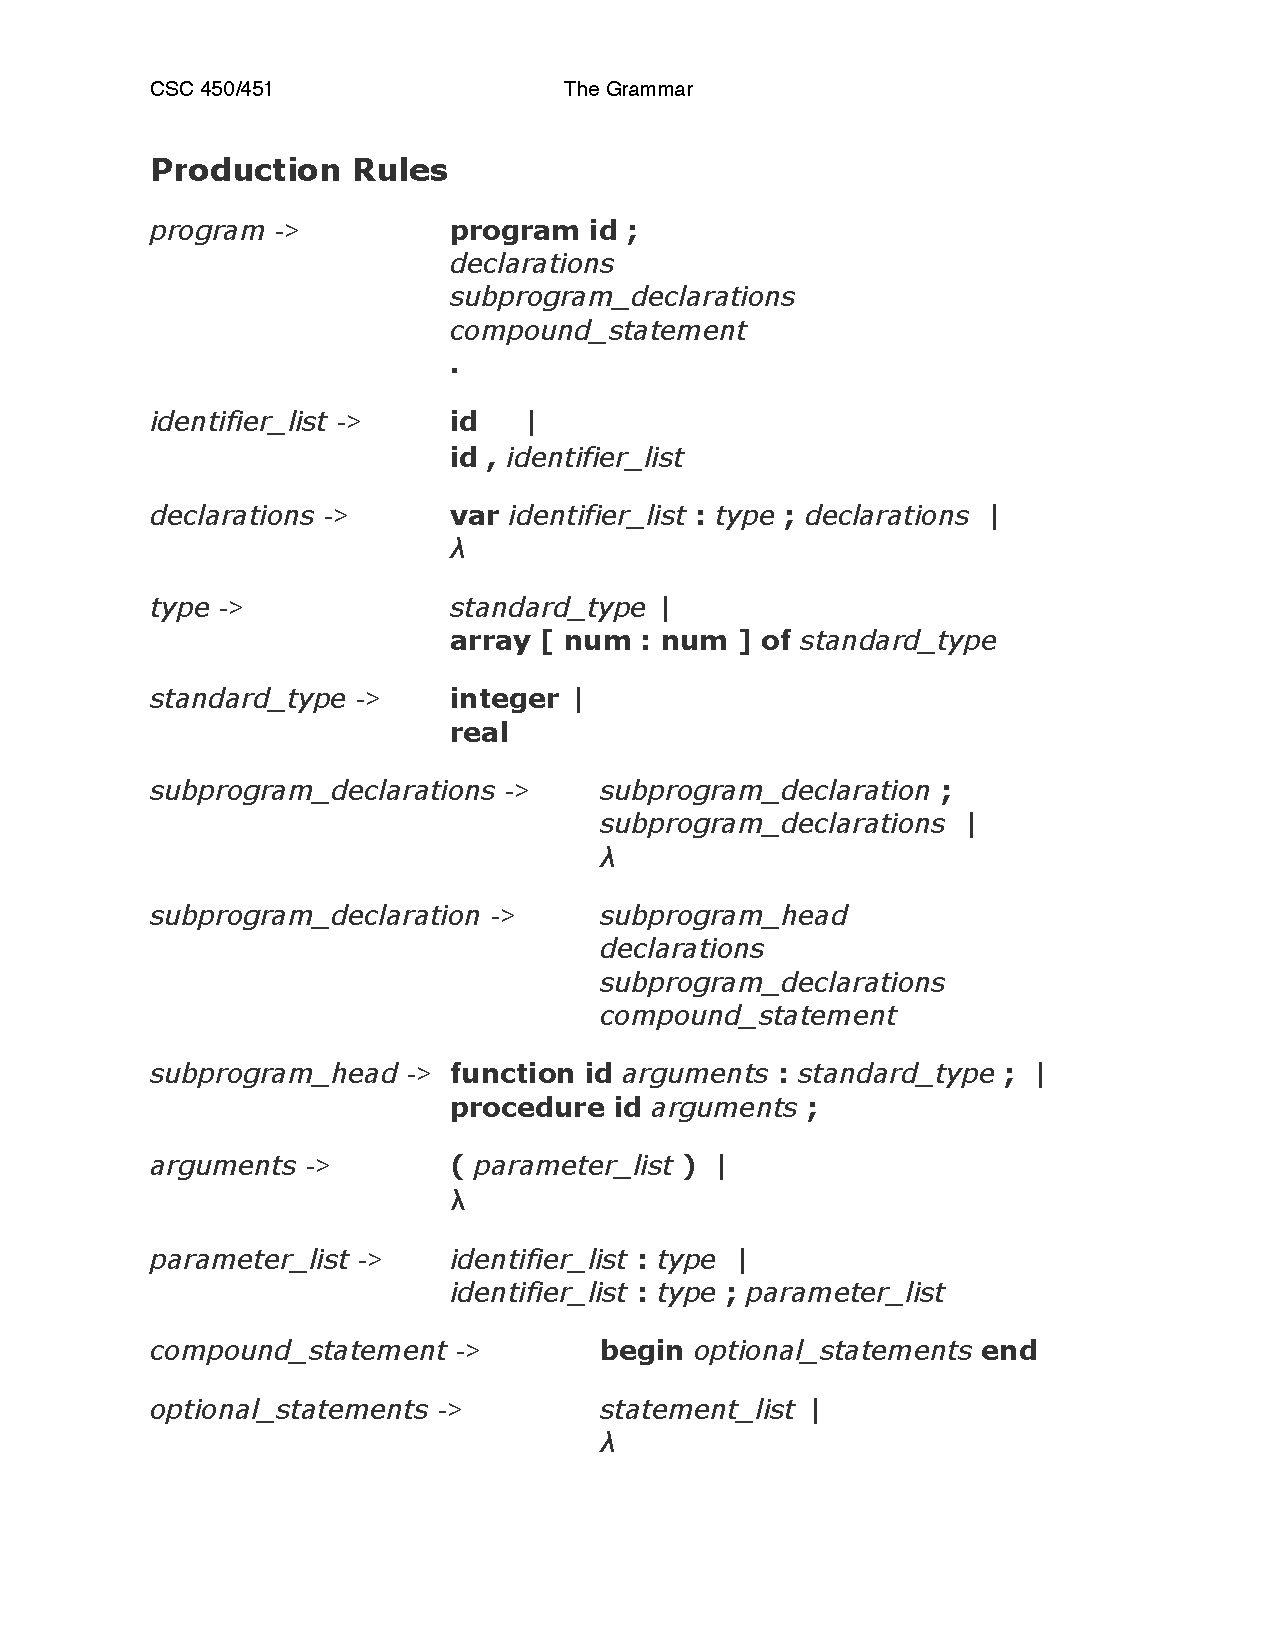
\includepdf[pages={1,2,3}]{Grammar.pdf}
\end{document}
